\begin{frame}{Etablering af skov}

\small

\begin{columns}[T]

\begin{column}{0.58\textwidth}

\textbf{Regler for etablering af skov:}

\begin{itemize}[]
\item Opfylder regler for skovrejsning
\item Skal opfylde kravene for tilskud under skovrejsningsordningerne
\item Tiltaget er pointgivende i 5 år fra anlæggelsesåret
\end{itemize}

\vspace{0.4em}

\textbf{Gavner arter:}

\footnotesize
Rådyr, dådyr, ræv, hare, fasan, rødrygget tornskade, gul vipstjert, 
pirol, gulspurv, blåmejse, musvit, sortmejse, grønsisken, stillits, rødhals, 
nattergal, hærfugl, flagermus, pindsvin, lækat, egern, musvåge, spurvehøg, 
tårnfalk, rørhøg, rådyr, kronvildt (senere stadier)

\end{column}

\begin{column}{0.40\textwidth}
\centering
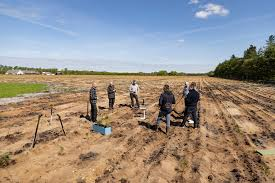
\includegraphics[width=\textwidth]{Billeder/Vildtforvaltning/biotopplantiltag/skovrejsning.jpeg}
\end{column}

\end{columns}

\end{frame}